\documentclass{beamer}
\usepackage{graphicx}
\usepackage{xcolor}
\usepackage{amssymb}
\usepackage{subcaption}
\newif\ifbeamer
\beamertrue

%further improvement
%background intro added Chen Chuan's work
%simulation add hierarchical method
%find suitable dataset to apply info-clustering
%Yang Li's suggestion: compared with other clustering method, the threshold is the same or not
%early stopping technique, complexity from n -> log(n)
\title{Research Progress Report}
\author{Feng Zhao}
\date{\today}
\begin{document}
\begin{frame}
	\titlepage
\end{frame}


\section{Introduction}

\begin{frame}
\frametitle{Problems}
Compute the probability content $P(H_n)$ of the convex hull $H_n$
of $n$ random points in $\mathbb{R}^d$
\begin{itemize}
\item the random points are i.i.d. sampled from a given distribution $\Gamma$
\item we are more interested in the asymptotic behavior of $P(H_n)$
as $n\to\infty$
\end{itemize}
\end{frame}
\begin{frame}
	\frametitle{Equivalent problem}
    \begin{align}
        P(H_n^c) & = \frac{1}{n+1}\mathbb{E}[V_{n+1}]\\
        F_{n+1} & = V_{n+1} (d-1) - d^2 + d + 2
    \end{align}   
    Therefore, we only need to integrate
    $\mathbb{E}[F_{n+1}]$
\end{frame}   
\begin{frame}
    \frametitle{Special cases}
    $d=1,P(H_n^c) = \frac{2}{n+1}$ for any distribution.
    
    Consider $d$ is fixed, $n\to \infty$.
    \begin{table}
        \begin{tabular}{|c|c|c|c|}
            \hline
            Distribution & $d=2$ & $d=3$ &  general $d$ \\
            \hline
            Uniform sphere & $C_2 n^{-1/3}$ & $C_3 n^{-1/2}$ &
            $C_{d} n^{-2/(d+1)}$ \\
            \hline
            Multivariate Gaussian &
            $2\sqrt{2\pi}\frac{\sqrt{\log n}}{n}$
            & $\frac{4\pi}{\sqrt{3}}\frac{\log n}{n}$ & $D_d\frac{(\log n)^{(d-1)/2}}{n}$ \\
            \hline
            Multivariate Cauchy & 
            \textcolor{red}{$\frac{\pi^2}{2}n^{-1}$} &
            \textcolor{red}{$\frac{2\pi^2}{3}n^{-1}$} &\\
            \hline
        \end{tabular}
        \caption{Asymptotic behavior of $P(H_n^c)$}
    \end{table}
    Some known constants:
    \begin{align*}
    C_2 &= \Gamma\left(\frac{5}{3}\right) \left(\frac{16\pi^2}{3}
    \right)^{1/3} \\
    C_3 &= \frac{35\sqrt{3\pi}}{12}
    \end{align*}
\end{frame}
\begin{frame}
    \frametitle{Simulation}
    The horizontal red line represents the theoretical coefficient.
    \begin{figure}
        \centering
        \begin{subfigure}[b]{0.5\linewidth}
        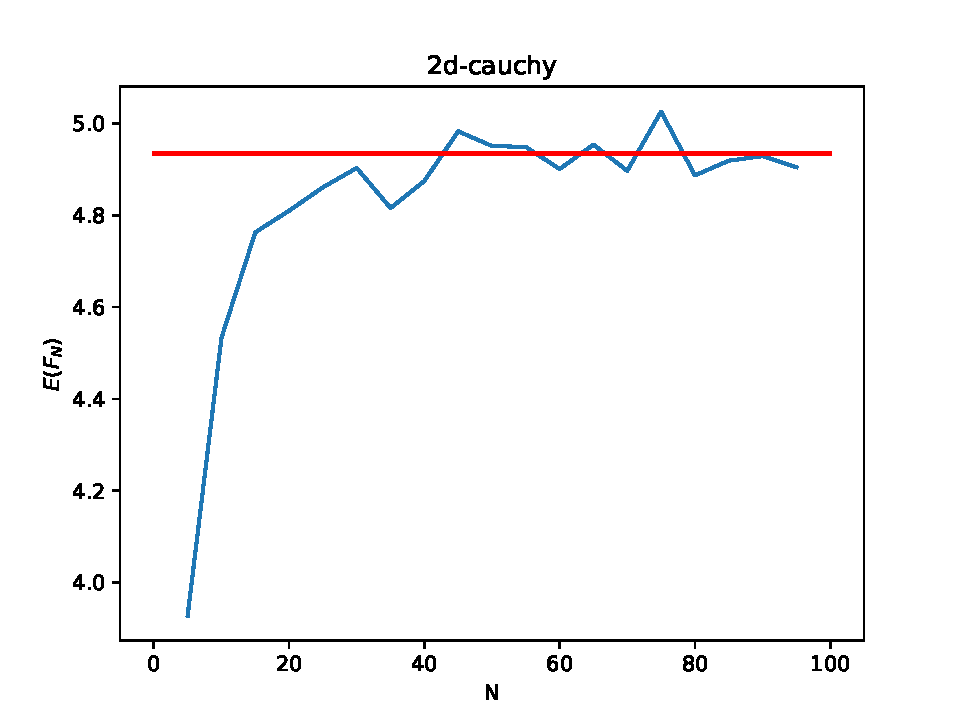
\includegraphics[width=\textwidth]{fig/2d-cauchy.pdf}
        \caption{$d=2$}
        \label{fig:2d_cauchy}
        \end{subfigure}~
        \begin{subfigure}[b]{0.5\linewidth}
          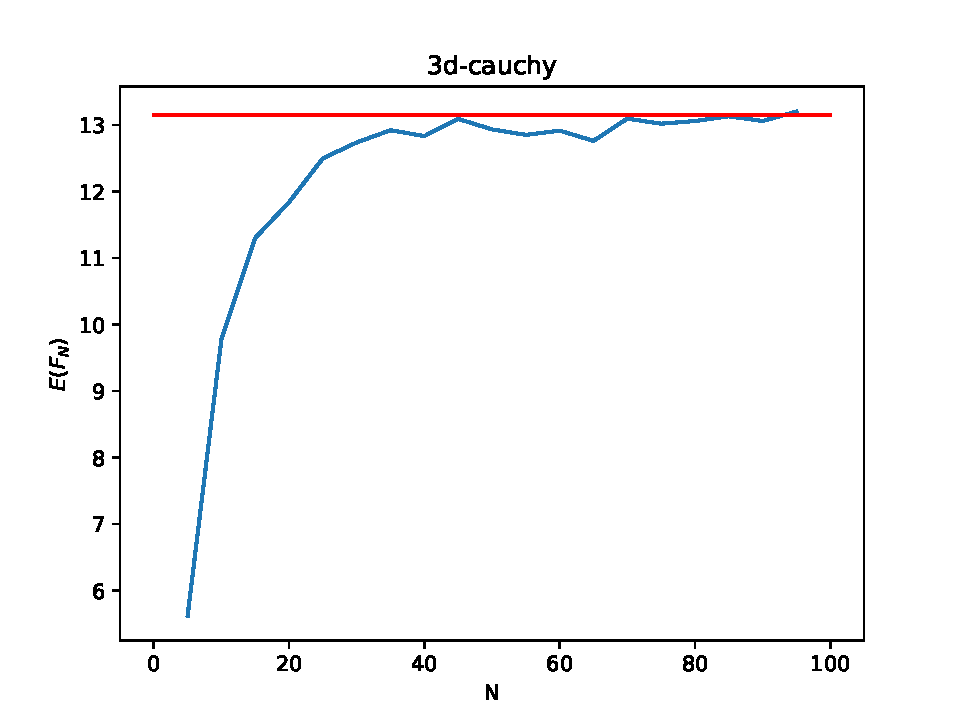
\includegraphics[width=\textwidth]{fig/3d-cauchy.pdf}
          \caption{$d=3$}
          \label{fig:3d_cauchy}
          \end{subfigure}
          \caption{The expected number of faces $E(F_N)$ varies with $n$}
      \end{figure}
\end{frame}
\end{document}
